\chapter{\IfLanguageName{dutch}{Stand van zaken}{State of the art}}%
\label{ch:stand-van-zaken}


% Tip: Begin elk hoofdstuk met een paragraaf inleiding die beschrijft hoe
% dit hoofdstuk past binnen het geheel van de bachelorproef. Geef in het
% bijzonder aan wat de link is met het vorige en volgende hoofdstuk.

% Pas na deze inleidende paragraaf komt de eerste sectiehoofding.

%Dit hoofdstuk bevat je literatuurstudie. De inhoud gaat verder op de inleiding, maar zal het onderwerp van de bachelorproef *diepgaand* uitspitten. De bedoeling is dat de lezer na lezing van dit hoofdstuk helemaal op de hoogte is van de huidige stand van zaken (state-of-the-art) in het onderzoeksdomein. Iemand die niet vertrouwd is met het onderwerp, weet nu voldoende om de rest van het verhaal te kunnen volgen, zonder dat die er nog andere informatie moet over opzoeken \autocite{Pollefliet2011}.

%Je verwijst bij elke bewering die je doet, vakterm die je introduceert, enz.\ naar je bronnen. In \LaTeX{} kan dat met het commando \texttt{$\backslash${textcite\{\}}} of \texttt{$\backslash${autocite\{\}}}. Als argument van het commando geef je de ``sleutel'' van een ``record'' in een bibliografische databank in het Bib\LaTeX{}-formaat (een tekstbestand). Als je expliciet naar de auteur verwijst in de zin (narratieve referentie), gebruik je \texttt{$\backslash${}textcite\{\}}. Soms is de auteursnaam niet expliciet een onderdeel van de zin, dan gebruik je \texttt{$\backslash${}autocite\{\}} (referentie tussen haakjes). Dit gebruik je bv.~bij een citaat, of om in het bijschrift van een overgenomen afbeelding, broncode, tabel, enz. te verwijzen naar de bron. In de volgende paragraaf een voorbeeld van elk.

%\textcite{Knuth1998} schreef een van de standaardwerken over sorteer- en zoekalgoritmen. Experten zijn het erover eens dat cloud computing een interessante opportuniteit vormen, zowel voor gebruikers als voor dienstverleners op vlak van informatietechnologie~\autocite{Creeger2009}.

%Let er ook op: het \texttt{cite}-commando voor de punt, dus binnen de zin. Je verwijst meteen naar een bron in de eerste zin die erop gebaseerd is, dus niet pas op het einde van een paragraaf.

Om het onderzoeksonderwerp samen met de achterliggende uitdaging te begrijpen, is het belangrijk om de werking van een Public Key Infrastructure (PKI) te begrijpen.
\textcite{Thales2025} definieert een PKI als een set van hardware, software, policies, processen en procedures die noodzakelijk zijn voor het maken, beheren, uitgeven, gebruiken, opslaan en intrekken van digitale certificaten en publieke keys.
PKI's zijn de basis die het gebruik van technologieëen zoals digitale handtekeningen en encryptie mogelijk maakt over een grote populatie van gebruikers.
Zij helpen namelijk met het vaststellen van de identiteit van personen, apparaten en diensten, wat gecontrolleerde toegang tot systemen en bronnen alsook data beveiliging en controle mogelijk maakt. \break

Een groot deel van PKI's zijn Digitale Certificaten en Certificate Authorities (CA's).
Een certificate authority is een bedrijf of organisatie die de identiteit van entiteiten (zoals websites, e-mail adressen, bedrijven, individuen, enz.) valideert en ze vastbindt aan cryptografische sleutels door middel van het uitgeven van electronische documenten gekend als digitale certificaten.
Deze certificaten brengen een aantal functionaliteiten zoals: authenticatie, Encryptie en integriteit.
Authenticatie: Een certificaat doet zich voor als een getuigschrift dat de identiteit valideert van de entiteit waaraan het is uitgegeven.
Encryptie: Een certificaat kan gebruikt worden voor beveiligde communicatie over onbeveiligde netwerken zoals het internet.
Integriteit: Een certificaat kan via digitale handtekeningen de integriteit van documenten verzekeren zodanig ze niet gewijzigd kunnen worden door een derde partij tijdens de transmissie.
Deze certificaten zorgen dus voor een beveiligde en geëncrypteerde communicatie tussen 2 partijen via public key cryptografie. \autocite{SSLcom} \break

\begin{figure}
  \centering
  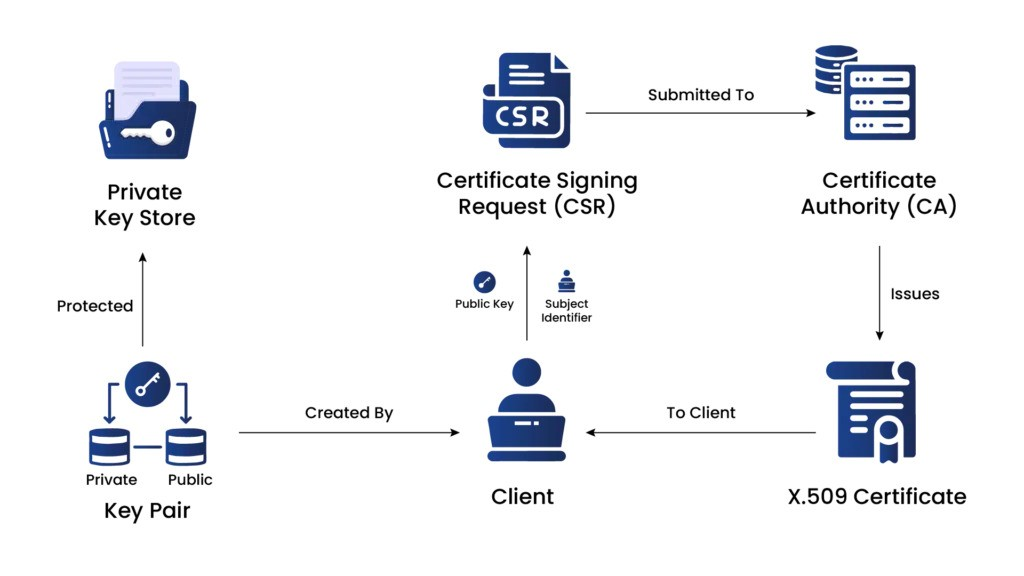
\includegraphics[width=0.8\textwidth]{CertEnr.jpg}
  \caption[Certificate enrollment.]{\label{fig:certenr}Deze afbeelding toont de stappen en componenten in het certificaat uitgave proces.}
\end{figure}

Wanneer een certificaat wordt aangevraagd bij een CA, moet de aanvrager eerst een public en private key genereren. De private key moet onder de controle en eigendom van de aanvrager blijven. In sommige gevallen worden de private keys gegenereerd en veilig bewaart in een Hardware Security Module (HSM) die behoort tot de CA. \autocite{SSLcom}
Om de registratie van certificaten te starten, maakt de aanvrager een Certificate Signing Request (CSR) aan. Deze CSR bevat de public key en andere informatie van de aanvrager die in het certificaat zal worden opgenomen, zoals de domeinnaam voor een SSL/TLS certificaat of de aanvrager's e-mail adres voor een S/MIME certificaat.
Daarna wordt de CSR ingedient bij de CA. De CA zal de identiteit van de aanvrager samen met de bijkomende informatie verifiëren. De CA kan verschillende manieren gebruiken om de aanvrager zijn identiteit te verifiëren, zoals e-mail verificatie, domein validatie of manuele validatie van juridische documenten.
Wanneer de CA het verificatie proces heeft voltooid en vaststelt dat de aanvrager legitiem is, zal het digitale certificaat worden uitgegeven. Het certificaat zal de aanvrager zijn public key en bijkomende informatie bevatten, alsook een geldigheidstermijn en de digitale handtekening van de CA.
Het uitgegeven certificaat wordt dan terug gebracht naar de aanvrager, afhankelijk van de CA en het certificaat type zal het certificaat geleverd worden op een verschillende manier zoals via e-mail, een beveiligd portaal of een andere methode.
Na het ontvangen van het certificaat is het aan de aanvrager om het certificaat te installeren op de toepasselijke server of apparaat waar het zal worden gebruikt. Als voorbeeld, een SSL/TLS certificaat wordt geïnstalleerd op een webserver voor een beveiligde connectie naar een website.
Eenmaal het certificaat is geïnstalleerd, kan het gebruikt worden voor protocolen die verantwoordelijk zijn voor beveiligde communicatie. Clients, gebruikers of andere entiteiten die in contact komen met de certificaat eigenaar kunnen de authenticiteit van het certificaat verifiëren aan de hand van de CA zijn digitale handtekening, wat een beveiligde en betrouwbare connectie verzekerd.
Zoals eerder vermeld hebben deze certificaten een geldigheidstermijn (meestal 1 tot 2 jaren). Voor ze vervallen, moet de aanvrager het certificaat vernieuwen via een gelijkaardig proces om het te kunnen blijven gebruiken zonder onderbrekingen. \autocite{EncCon} \break

Het verifiëren van een certificaat om de bepalen of het vertrouwd kan worden is belangrijk voor de veiligheid van de communicatie.
\Textcite{okta} zegt dat tijdens een SSL/TLS handshake, de client het certificaat van de server ontvangt. De client controleert of het certificaat nog niet vervallen is en dat de domeinnaam en IP adres op het certificaat gelijkaardig zijn aan dat van de server. Daarna zal de client kijken of het certificaat correct is ondertekend door een vertrouwde CA.
In de meeste gevallen zal de server certificate niet ondertekend zijn door de root CA die door de client wordt vertrouwd. In plaats van de root CA zal de client 1 of meerdere intermediate CA's vertrouwen zolang als hun ketting van vertrouwen terug leidt naar een root CA die de client vertrouwd.

Voor elke intermediate CA certificate doet de client hetzelfde verificatie proces waarbij de uitgever (issuer) zijn naam overeenkomt met de certificate eigenaar zijn naam van de volgende certificate in de ketting. Ook wordt de digitale signatuur en public key van het certificaat bekeken om te kijken of deze correct is ondertekend.
Dit proces herhaald zichzelf tot de client komt bij een self-signed root CA certificate die de client vertrouwd.
Op dit moment heeft de client dan een cryptografische ketting van vertrouwen gemaakt tot de server en kan de SSL/TLS handshake verder gaan. \break
\begin{figure}
  \centering
  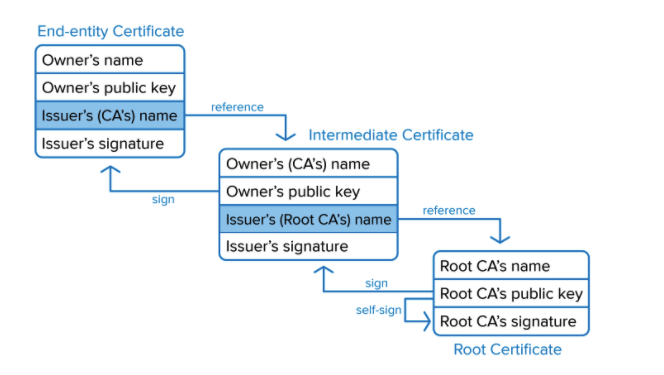
\includegraphics[width=0.8\textwidth]{chainoftrust.png}
  \caption[Chain of trust]{\label{fig:chainoftrust}Deze afbeelding toont de ketting van vertrouwen die de client nakijkt tijdens het verifiëren van een certificaat.}
\end{figure}

Bij dit verificatie proces eindigt de client steeds bij een root CA certificaat die door de client moet worden vertrouwd. Om te bepalen welke root CA's door de client worden vertrouwd bestaan er trust stores.
Een trust store is een collectie van root certificaten die standaard worden vertrouwd door een client en worden beheerd door bedrijven die de client zijn operating system of browser ontwikkelen, zoals Microsoft, Mozilla en Google.
Elke vendor heeft zijn eigen standaarden voor root certificaten maar ze vereisen allemaal dat een uitgevende CA een of meerdere controles ondergaan om hun vertrouwbaarheid, validiteit en conformiteit vast te stellen via de CA/B Forum Baseline Requirements vooraleer ze worden opgenomen in hun trust store. \autocite{Venafi}
Over al de trust stores van deze vendors zijn er heel wat certificaten die niet noodzakelijk zijn. Een studie van \textcite{PerlHenning} toont dat alleen maar 66\% van de certificaten in de trust store van Windows, Linux, MacOS, Firefox, iOS and Android noodzakelijk zijn voor het vertrouwen van websites.
Dit zorgt ervoor dat de overige derde van de root certificaten in de trust stores een potentieel veiligheidsrisico vormen voor de client. \break

Als oplossing hierop kunnen bedrijven het overwegen om deze standaard trust stores af te wijzen. In de plaats daarvan kunnen ze best hun eigen aangepaste, corporate-level trust store maken en gebruik maken van certificate white-listing om te bepalen welke root certificates hierin kunnen opgenomen worden.
Dit helpt bedrijven met het aanvals oppervlak te verkleinen door het limiteren van de hoeveelheid vertrouwde CA's en het markeren van niet-vertrouwde SSL/TLS sessies.
Organisaties kunnen dan deze certificate whitelist en blacklist updaten op een regelmatige basis afhankelijk van benoodigdheden van hun evoluerende business requirements en groeiend CA landschap. \autocite{Venafi} 

Het beheren van deze trust stores kan een uitdaging zijn voor bedrijven, zeker bedrijven met heterogene netwerken (netwerken die clients hebben met verschillende operating systemen en browsers).
\textcite{rfc6024} weerlegt dit door te zeggen dat deze trust anchors (Root CA certificaten) vaak bewaart worden in applicatie-specifieke of OS-specifieke trust stores.
Vaak heeft dan 1 machine een verschillend aantal trust stores die niet gesynchroniseerd zijn met elkaar. \break

De uitdagingen hier zijn dus het vermijden van overbodige vertrouwde root certificaten binnen een netwerk en zijn segmenten afhankelijk van de business requirements en het beheren van deze trust stores over verschillende machines en applicaties. 

%\begin{figure}
%  \centering
%  \includegraphics[width=0.8\textwidth]{grail.jpg}
%  \caption[Voorbeeld figuur.]{\label{fig:grail}Voorbeeld van invoegen van een figuur. Zorg altijd voor een uitgebreid bijschrift dat de figuur volledig beschrijft zonder in de tekst te moeten gaan zoeken. Vergeet ook je bronvermelding niet!}
%\end{figure}

%\begin{listing}
%  \begin{minted}{python}
%    import pandas as pd
%    import seaborn as sns
%
%    penguins = sns.load_dataset('penguins')
%    sns.relplot(data=penguins, x="flipper_length_mm", y="bill_length_mm", hue="species")
%  \end{minted}
%  \caption[Voorbeeld codefragment]{Voorbeeld van het invoegen van een codefragment.}
%\end{listing}

%\lipsum[7-20]

%\begin{table}
%  \centering
%  \begin{tabular}{lcr}
%    \toprule
%    \textbf{Kolom 1} & \textbf{Kolom 2} & \textbf{Kolom 3} \\
%    $\alpha$         & $\beta$          & $\gamma$         \\
%    \midrule
%    A                & 10.230           & a                \\
%    B                & 45.678           & b                \\
%    C                & 99.987           & c                \\
%    \bottomrule
%  \end{tabular}
%  \caption[Voorbeeld tabel]{\label{tab:example}Voorbeeld van een tabel.}
%\end{table}

